\documentclass[
11pt, % The default document font size, options: 10pt, 11pt, 12pt
codirector, % Uncomment to add a codirector to the title page
]{charter} 




% El títulos de la memoria, se usa en la carátula y se puede usar el cualquier lugar del documento con el comando \ttitle
\titulo{Desarrollo de un dispositivo de rastreo satelital mediante GNSS (Global Navigation Satellite System)} 

% Nombre del posgrado, se usa en la carátula y se puede usar el cualquier lugar del documento con el comando \degreename
\posgrado{Carrera de Especialización en Sistemas Embebidos} 
%\posgrado{Carrera de Especialización en Internet de las Cosas} 
%\posgrado{Carrera de Especialización en Intelegencia Artificial}
%\posgrado{Maestría en Sistemas Embebidos} 
%\posgrado{Maestría en Internet de las cosas}

% Tu nombre, se puede usar el cualquier lugar del documento con el comando \authorname
\autor{Ing. Nicolás Gabriel Cettra} 

% El nombre del director y co-director, se puede usar el cualquier lugar del documento con el comando \supname y \cosupname y \pertesupname y \pertecosupname
\director{Nombre del Director}
\pertenenciaDirector{pertenencia} 
% FIXME:NO IMPLEMENTADO EL CODIRECTOR ni su pertenencia
\codirector{John Doe} % para que aparezca en la portada se debe descomentar la opción codirector en el documentclass
\pertenenciaCoDirector{FIUBA}

% Nombre del cliente, quien va a aprobar los resultados del proyecto, se puede usar con el comando \clientename y \empclientename
\cliente{Alejandro Castellano}
\empresaCliente{America GIS S.R.L.}

% Nombre y pertenencia de los jurados, se pueden usar el cualquier lugar del documento con el comando \jurunoname, \jurdosname y \jurtresname y \perteunoname, \pertedosname y \pertetresname.
\juradoUno{Nombre y Apellido (1)}
\pertenenciaJurUno{pertenencia (1)} 
\juradoDos{Nombre y Apellido (2)}
\pertenenciaJurDos{pertenencia (2)}
\juradoTres{Nombre y Apellido (3)}
\pertenenciaJurTres{pertenencia (3)}
 
\fechaINICIO{21 de junio de 2023}		%Fecha de inicio de la cursada de GdP \fechaInicioName
\fechaFINALPlan{15 de agosto de 2023} 	%Fecha de final de cursada de GdP
\fechaFINALTrabajo{15 de mayo de 2024}	%Fecha de defensa pública del trabajo final


\begin{document}

\maketitle
\thispagestyle{empty}
\pagebreak


\thispagestyle{empty}
{\setlength{\parskip}{0pt}
\tableofcontents{}
}
\pagebreak


\section*{Registros de cambios}
\label{sec:registro}


\begin{table}[ht]
\label{tab:registro}
\centering
\begin{tabularx}{\linewidth}{@{}|c|X|c|@{}}
\hline
\rowcolor[HTML]{C0C0C0} 
Revisión & \multicolumn{1}{c|}{\cellcolor[HTML]{C0C0C0}Detalles de los cambios realizados} & Fecha      \\ \hline
0      & Creación del documento                                 &\fechaInicioName \\ \hline
1      & Se completa hasta el punto 5 inclusive                 & 04 de julio de 2023 \\ \hline
2      & Se completa hasta el punto 9 inclusive                 & 10 de julio de 2023 \\ \hline
3      & Se completa hasta el punto 12 inclusive                & 20 de julio de 2023 \\ \hline
3      & Se completa hasta el punto 15 inclusive                & 28 de julio de 2023 \\ \hline
%		  Se puede agregar algo más \newline
%		  En distintas líneas \newline
%		  Así                                                    & dd/mm/aaaa \\ \hline
%3      & Se completa hasta el punto 11 inclusive                & dd/mm/aaaa \\ \hline
%4      & Se completa el plan	                                 & dd/mm/aaaa \\ \hline
\end{tabularx}
\end{table}

\pagebreak



\section*{Acta de constitución del proyecto}
\label{sec:acta}

\begin{flushright}
Buenos Aires, \fechaInicioName
\end{flushright}

\vspace{2cm}

Por medio de la presente se acuerda con el Ing. \authorname\hspace{1px} que su Trabajo Final de la \degreename\hspace{1px} se titulará ``\ttitle'', consistirá esencialmente en la implementación de un sistema embebido que tendrá la capacidad de adquirir posicionamiento satelital. Este sistema podrá comunicarse con el servidor proporcionado por la organización mediante internet. Además, contará con un acelerómetro para detectar aceleraciones repentinas en el dispositivo, un botón de propósito general y una autonomía de al menos 24 horas; y tendrá un presupuesto preliminar estimado de 612 horas de trabajo y 7065 USD, con fecha de inicio \fechaInicioName\hspace{1px} y fecha de presentación pública \fechaFinalName.

Se adjunta a esta acta la planificación inicial.

\vfill

% Esta parte se construye sola con la información que hayan cargado en el preámbulo del documento y no debe modificarla

\begin{table}[ht]
\centering
\begin{tabular}{ccc}
\begin{tabular}[c]{@{}c@{}}Dr. Ing. Ariel Lutenberg \\ Director posgrado FIUBA\end{tabular} & \hspace{2cm} & \begin{tabular}[c]{@{}c@{}}\clientename \\ \empclientename \end{tabular} \vspace{2.5cm} \\ 
\multicolumn{3}{c}{\begin{tabular}[c]{@{}c@{}} \supname \\ Director del Trabajo Final\end{tabular}} \vspace{2.5cm} \\
%\begin{tabular}[c]{@{}c@{}}\jurunoname \\ Jurado del Trabajo Final\end{tabular}     &  & \begin{tabular}[c]{@{}c@{}}\jurdosname\\ Jurado del Trabajo Final\end{tabular}  \vspace{2.5cm}  \\
%\multicolumn{3}{c}{\begin{tabular}[c]{@{}c@{}} \jurtresname\\ Jurado del Trabajo Final\end{tabular}} \vspace{.5cm}                                                                     
\end{tabular}
\end{table}


\section{1. Descripción técnica-conceptual del proyecto a realizar}
\label{sec:descripcion}


Con el objetivo de ofrecer soluciones más específicas de manera flexible y económica, se desarrollará un sistema embebido que permitirá adquirir un posicionamiento global a través de un módulo GNSS. Este sistema se comunicará con el servidor proporcionado por la organización mediante GPRS. Además, contará con un acelerómetro para detectar aceleraciones bruscas en el dispositivo. También se incluirá un botón con funciones programables de propósito múltiple y una autonomía de al menos 24 horas.

Una de las características clave que se debe tener en cuenta es la capacidad de adaptar el hardware a diferentes sectores. Para el desarrollo de este dispositivo, se utilizará el módulo GNSS/GPRS A9G de la empresa Ai Thinker, al que se le acoplará el hardware necesario para cumplir con los objetivos planteados. Es importante mencionar que se cuenta con el SDK del módulo, lo que permitirá programarlo según las necesidades.

El dispositivo debe ser capaz de enviar información a través de GPRS utilizando los protocolos de comunicación UDP o TCP, y se requerirá la capacidad de utilizar MQTT dentro del protocolo TCP. Dicha comunicación se puede apreciar en la figura 1. Además, se utilizará el acelerómetro MPU6050 mediante la interfaz I2C para la adquisición de aceleraciones.

En cuanto a la alimentación del dispositivo, se utilizará una batería de 3,7 V. Esto hace que la eficiencia energética sea indispensable para maximizar la duración de la batería.

En cuanto al botón, este debe ser multiproposito. El dispositivo generará un evento al pulsarlo y el significado será asignado del lado del servidor.

El software embebido debe ser diseñado teniendo en cuenta la posibilidad de agregar módulos adicionales en el futuro, y se implementará un sistema operativo en tiempo real (RTOS). Además, se utilizará como base para futuros proyectos.

En la figura 1 se puede apreciar el diagrama en bloques de la comunicación entre el dispositivo y el servidor.


\begin{figure}[htpb]
\centering 
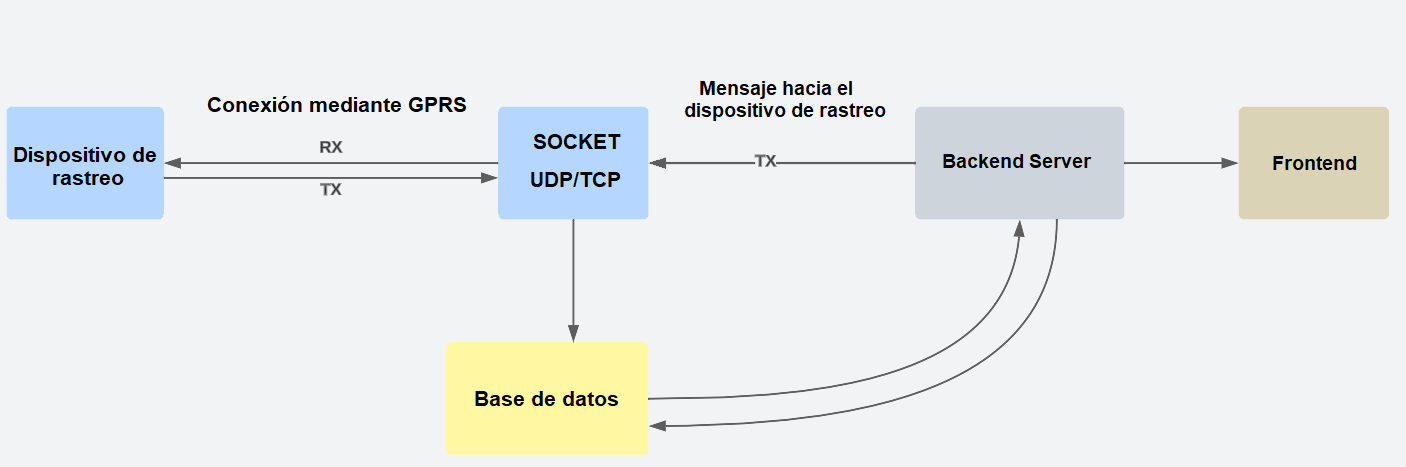
\includegraphics[width=1\textwidth]{./Figuras/diagBloque.png}
\caption{Diagrama en bloques del sistema.}
\label{fig:diagBloques}
\end{figure}

\vspace{30px}
\pagebreak
\section{2. Identificación y análisis de los interesados}
\label{sec:interesados}


\begin{table}[ht]
%\caption{Identificación de los interesados}
%\label{tab:interesados}
\begin{tabularx}{\linewidth}{@{}|l|X|X|l|@{}}
\hline
\rowcolor[HTML]{C0C0C0} 
Rol           & Nombre y Apellido & Organización 	& Puesto 	\\ \hline
Cliente       & \clientename      &\empclientename	&    Gerente    	\\ \hline
Responsable   & \authorname       & FIUBA        	& Alumno 	\\ \hline
Orientador    & \supname	      & \pertesupname 	& Director Trabajo final \\ \hline
Usuario final    & Público en general	      & - 	& - \\ \hline
\end{tabularx}
\end{table}

\section{3. Propósito del proyecto}
\label{sec:proposito}


El propósito de este proyecto es desarrollar un sistema embebido que permita controlar un hardware de adquisición de datos, en particular enfocado en el posicionamiento global. Se busca que este sistema tenga la capacidad de adaptarse a diferentes sectores, brindando flexibilidad y versatilidad en su aplicación. Además, se busca lograr una solución más económica en comparación con otras alternativas disponibles en el mercado. El enfoque central es garantizar la adaptabilidad del hardware y reducir los costos asociados al desarrollo y despliegue del sistema.


\section{4. Alcance del proyecto}
\label{sec:alcance}

El sistema embebido a desarrollar tendrá los siguientes alcances: \\

El proyecto incluye:
\begin{itemize}

    \item Implementación en RTOS de bibliotecas para la interpretación de tramas GPS y el protocolo de comunicación con control CRC (verificación por redundancia cíclica).
    \item Desarrollo del protocolo para el envio de reportes gatillados por eventos.
    \item Desarrollo del kit de comandos para configurar el dispositivo mediante USB, GPRS o SMS.
    \item Desarrollo del software que sea capaz de establecer una conexión a Internet mediante GPRS para el intercambio de información via UDP/TCP.
    \item Implementacion del software para que sea capaz de gestionar reportes en memoria en caso de interrupciones en la conexión a Internet.
    \item Elaboración de manuales de usuario, guías rápidas de uso y otros materiales de documentación.

\end{itemize}
El proyecto no incluye:
\begin{itemize}
    \item Desarrollo del hardware.
    \item Calibraciones y certificaciones.
    \item Despliegue de la red de cobertura de la señal.
\end{itemize}
\pagebreak

\section{5. Supuestos del proyecto}
\label{sec:supuestos}
Para el desarrollo del presente proyecto se supone que:
\begin{itemize}
\item La empresa America GIS proporcionará el servidor encargado de recibir la información enviada por el dispositivo.
\item La empresa proporcionará el hardware necesario, incluyendo la tarjeta SIM para la conexión GPRS y la interfaz de programación del dispositivo.
\item El módulo GNSS en condiciones óptimas, tiene una tolerancia de error de 10 metros en la precisión de la posición.
\item El dispositivo solo funcionará si hay una antena compatible con 2G dentro de su rango de alcance.
\end{itemize}

\section{6. Requerimientos}
\label{sec:requerimientos}

\begin{enumerate}
\item Requerimientos funcionales
    \begin{enumerate}
    \item El sistema debe ser capaz de adquirir el posicionamiento global mediante un módulo GNSS.
    \item El sistema debe comunicarse con el servidor proporcionado por la empresa America GIS a través de GPRS.
    \item El dispositivo debe contar con un acelerómetro para detectar aceleraciones abruptas.
    \item El sistema debe tener un botón de propósito general con funcionalidad programable.
    \item El sistema debe tener una autonomía mínima de 24 horas.
    \item El sistema debe generar reportes temporizados.
    \item El sistema debe generar reportes en función de eventos particulares, como presionar el botón multipropósito, una aceleración abrupta o un cambio de dirección.
    \item El sistema debe ser configurable mediante USB, GPRS o SMS.
    \item El dispositivo debe conectarse a Internet mediante GPRS para el intercambio de información.
    \item El sistema debe ser capaz de comunicarse utilizando los protocolos UDP o TCP.
    \item El sistema debe ser capaz de almacenar reportes en memoria en caso de intermitencia en la conexión a Internet.
    \end{enumerate}

\item Requerimientos de documentación
    \begin{enumerate}
    \item Se debe proporcionar documentación detallada del proceso de configuración del sistema.
    \item Se debe incluir documentación del hardware utilizado, incluyendo el módulo GNSS, el acelerómetro y el botón multipropósito.
    \item Se debe proporcionar documentación del SDK del módulo GNSS/GPRS A9G de Ai Thinker.
    \item Se debe incluir una guía de usuario que explique el funcionamiento y las características del sistema.
    \item Se debe documentar el protocolo de comunicación utilizado para la interacción con el servidor de America GIS.
    \item Se debe proporcionar una documentación clara sobre las especificaciones y limitaciones del sistema, incluyendo la tolerancia de error del módulo GNSS y la dependencia de una antena compatible con 2G.
    \item Se debe proporcionar una memoria del trabajo.
    \item Se debe proporcionar un registro de avances.
    \end{enumerate}
\end{enumerate}

\section{7. Historias de usuarios (\textit{Product backlog})}
\label{sec:backlog}

En esta sección se presentarán las historias de usuario, y cada una de ellas recibirá una puntuación basada en tres aspectos:
\begin{itemize}
 \item Dificultad: representa la cantidad de trabajo necesario para completar la historia de usuario.
 \item Complejidad: indica la complejidad del trabajo requerido para cumplir con la historia de usuario.
 \item Riesgo: refleja el nivel de incertidumbre asociado con el trabajo necesario para la historia de usuario.
\end{itemize}
Se utilizará una escala basada en la serie de Fibonacci, donde los números mayores implicarán un mayor costo en términos de tiempo y recursos. Si la suma de los tres componentes no corresponde a un número de la serie de Fibonacci, se elegirá el número más cercano en la serie como puntuación asignada.

\begin{itemize}
    \item Como usuario, quiero poder configurar la frecuencia de generación de reportes temporizados para adaptarla a mis necesidades. (Ponderación: 5 story points)
    \begin{itemize}
        \item Dificultad: 2 (Moderada)
        \item Complejidad: 2 (Moderada)
        \item Riesgo: 1 (Bajo)
    \end{itemize}    
    
    \item Como usuario, quiero recibir notificaciones inmediatas en caso de detectar una aceleración abrupta en el dispositivo para poder tomar medidas rápidamente. (Ponderación: 10 story points)
    \begin{itemize}
        \item Dificultad: 3 (Compleja)
        \item Complejidad: 3 (Compleja)
        \item Riesgo: 4 (Alto)
    \end{itemize}    

    
    \item Como usuario, quiero poder personalizar la funcionalidad del botón multipropósito para adaptarlo a mis necesidades específicas. (Ponderación: 3 story points)
    \begin{itemize}
        \item Dificultad: 1 (Baja)
        \item Complejidad: 1 (Baja)
        \item Riesgo: 1 (Baja)
    \end{itemize}    

    
    \item Como usuario, quiero tener la opción de enviar los reportes de manera automática al servidor de America GIS a través del protocolo UDP para una comunicación más eficiente. (Ponderación: 8 story points)
    \begin{itemize}
        \item Dificultad: 2 (Moderada)
        \item Complejidad: 3 (Compleja)
        \item Riesgo: 3 (Moderado)
    \end{itemize}  
    
    \item Como usuario, quiero poder almacenar los reportes en memoria en caso de pérdida temporal de conexión a Internet para asegurar que no se pierda información importante. (Ponderación: 6 story points)
    \begin{itemize}
        \item Dificultad: 2 (Moderada)
        \item Complejidad: 2 (Moderada)
        \item Riesgo: 2 (Moderado)
    \end{itemize}  

    
    \item Como usuario, quiero recibir una notificación en tiempo real cuando se produzca un cambio de dirección brusco en el dispositivo para estar al tanto de cualquier evento inesperado. (Ponderación: 8 story points)
    \begin{itemize}
        \item Dificultad: 2 (Moderada)
        \item Complejidad: 3 (Compleja)
        \item Riesgo: 3 (Moderado)
    \end{itemize}  
    
    \item Como usuario, quiero tener la posibilidad de configurar el sistema mediante una interfaz sencilla y amigable a través de USB para facilitar la configuración y personalización. (Ponderación: 5 story points)
    \begin{itemize}
        \item Dificultad: 2 (Moderada)
        \item Complejidad: 2 (Moderada)
        \item Riesgo: 1 (Bajo)
    \end{itemize}  
    
    \item Como usuario, quiero poder consultar la documentación detallada del sistema para comprender mejor su funcionamiento y aprovechar al máximo sus características. (Ponderación: 3 story points)
    \begin{itemize}
        \item Dificultad: 1 (Baja)
        \item Complejidad: 1 (Baja)
        \item Riesgo: 1 (Bajo)
    \end{itemize}  
\end{itemize}


\section{8. Entregables principales del proyecto}
\label{sec:entregables}

Los entregables del proyecto son:
\begin{itemize}
    \item Manual de uso.
    \item Código fuente del firmware.
    \item Archivo binario para actualizar el dispositivo.
    \item Informe final.
\end{itemize}


\section{9. Desglose del trabajo en tareas}
\label{sec:wbs}


\begin{enumerate}
    \item Configuración inicial del entorno de desarrollo.
    \begin{enumerate}
        \item Instalación y configuración del software de desarrollo. (12 h)
        \item Configuración del entorno de programación y depuración. (12 h)
        \item Configuración del entorno de pruebas y simulación. (12 h)
    \end{enumerate}
    
    \item Desarrollo del módulo de adquisición de posicionamiento.
    \begin{enumerate}
        \item Investigación del módulo GNSS. (30 h)
        \item Implementación de la comunicación con el módulo GNSS. (30 h)
        \item Integración de la funcionalidad de posicionamiento en el sistema embebido. (36 h)
    \end{enumerate}
    
    \item Desarrollo del módulo de detección de aceleraciones abruptas.
    \begin{enumerate}
        \item Investigación del modulo acelerómetro. (24 h)
        \item Implementación de la lectura y procesamiento de datos del acelerómetro. (24 h)
        \item Integración de la detección de aceleraciones en el sistema embebido. (30 h)
    \end{enumerate}
    
    \item Desarrollo del módulo de configuración y personalización.
    \begin{enumerate}
        \item Diseño de la interfaz de configuración mediante USB. (24 h)
        \item Implementación de la comunicación y la lógica de configuración. (30 h)
        \item Pruebas y depuración de la funcionalidad de configuración. (24 h)
    \end{enumerate}
    
    \item Desarrollo del módulo de generación y envío de reportes.
    \begin{enumerate}
        \item Diseño e implementación de la generación de reportes temporizados. (36 h)
        \item Implementación de GPIO y la lógica de configuración. (18h)
        \item Desarrollo de la lógica para generar reportes en función de eventos. (30 h)
        \item Implementación de la comunicación con el servidor de America GIS. (36 h)
    \end{enumerate}
    
    \item Pruebas y validación del sistema completo.
    \begin{enumerate}
        \item Realización de pruebas de integración y validación del sistema embebido. (54 h)
        \item Pruebas de conectividad y comunicación con el servidor. (24 h)
        \item Pruebas de rendimiento y estabilidad del sistema. (24 h)
    \end{enumerate}
    
    \item Documentación del manual.
    \begin{enumerate}
        \item Elaboración del manual de usuario. (24 h)
        \item Revisión y edición del manual de usuario. (12 h)
    \end{enumerate}
    
    \item Elaboración del informe.
    \begin{enumerate}
        \item Recopilación y análisis de los resultados del proyecto. (24 h)
        \item Redacción del informe final. (30 h)
        \item Revisión y edición del informe final. (12 h)
    \end{enumerate}
\end{enumerate}

Cantidad total de horas estimadas: 612 h

\pagebreak
\section{10. Diagrama de Activity On Node}
\label{sec:AoN}

\begin{figure}[htpb]
\centering 
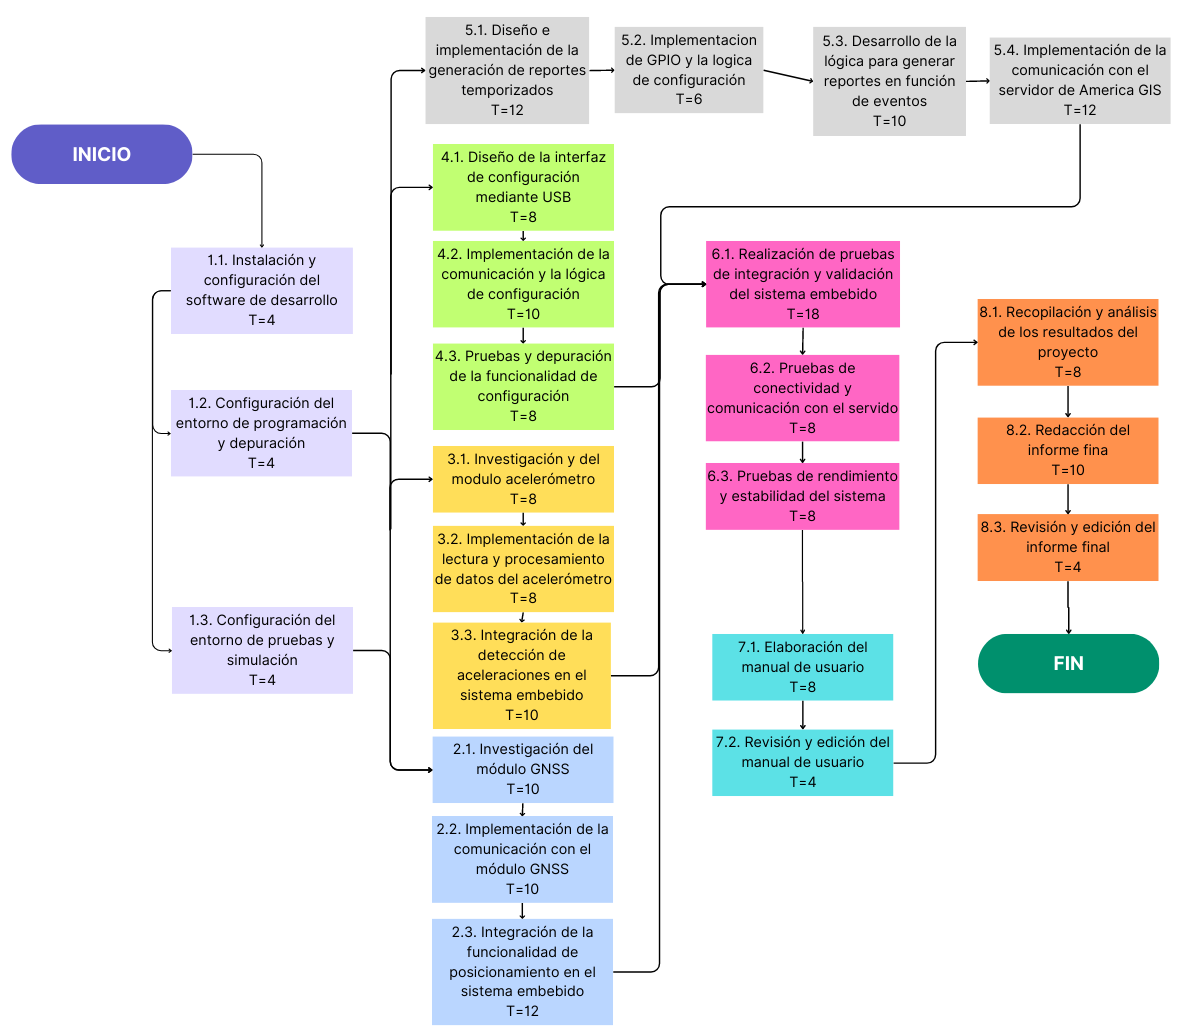
\includegraphics[width=1\textwidth]{./Figuras/diagrama1.png}
\caption{Diagrama de \textit{Activity on Node}.}
\label{fig:AoN}
\end{figure}
\pagebreak

\begin{figure}[htpb]
\centering 
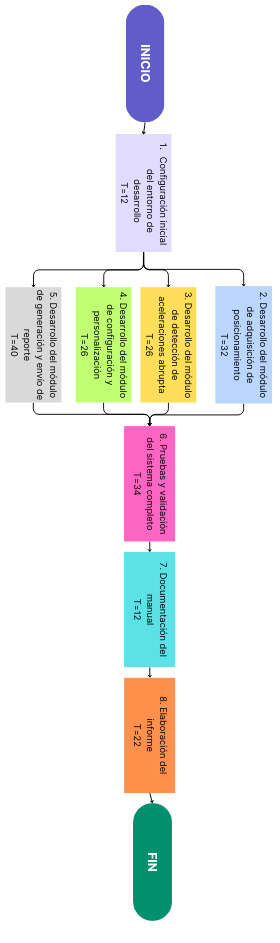
\includegraphics[width=.35\textwidth]{./Figuras/diagrama2rot.png}
\caption{Diagrama de \textit{Activity on Node agrupado}.}
\label{fig:AoN}
\end{figure}
\pagebreak

\section{11. Diagrama de Gantt}
\label{sec:gantt}
\begin{figure}[htpb]
\centering 
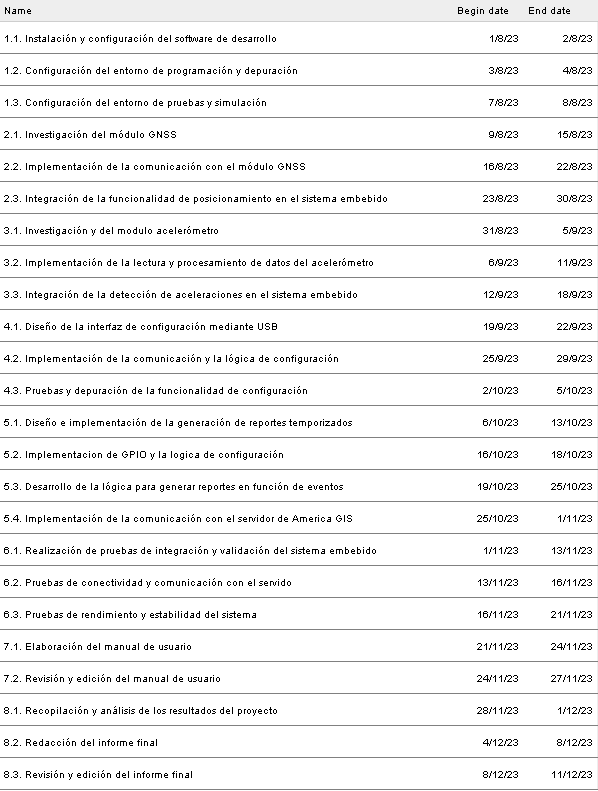
\includegraphics[height=0.75\textheight]{./Figuras/gantt_rotado2.png}
\caption{Diagrama de Gantt}

\label{fig:diagGantt}
\end{figure}
\pagebreak

\begin{figure}[htpb]
\centering 

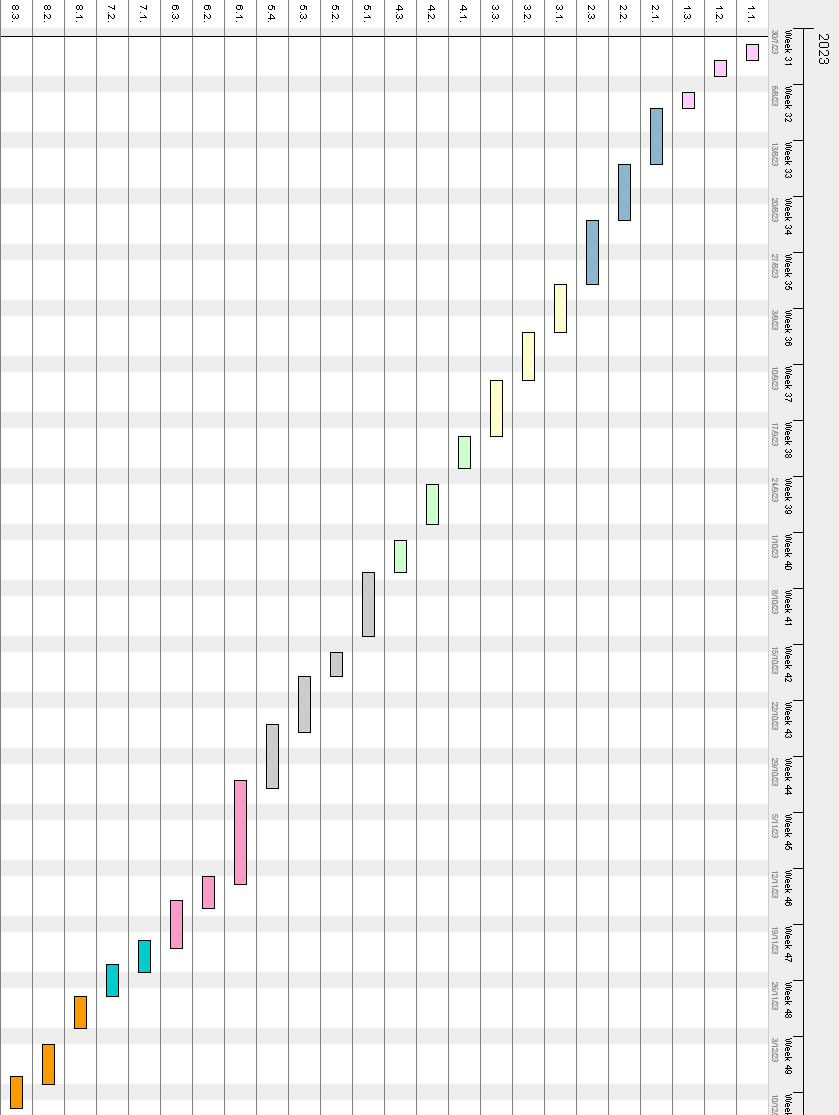
\includegraphics[height=0.78\textheight]{./Figuras/ganttRotado5.png}


\label{fig:diagGantt}
\end{figure}
\pagebreak

\section{12. Presupuesto detallado del proyecto}
\label{sec:presupuesto}

Los costos se encuentran expresados en USD.
\begin{table}[htpb]
\centering
\begin{tabularx}{\linewidth}{@{}|X|c|r|r|@{}}
\hline
\rowcolor[HTML]{C0C0C0} 
\multicolumn{4}{|c|}{\cellcolor[HTML]{C0C0C0}COSTOS DIRECTOS} \\ \hline
\rowcolor[HTML]{C0C0C0} 
Descripción &
  \multicolumn{1}{c|}{\cellcolor[HTML]{C0C0C0}Cantidad} &
  \multicolumn{1}{c|}{\cellcolor[HTML]{C0C0C0}Valor unitario} &
  \multicolumn{1}{c|}{\cellcolor[HTML]{C0C0C0}Valor total} \\ \hline
  \multicolumn{1}{|l|}{Dispositivo de rastreo}
 &
  \multicolumn{1}{c|}{ 1 } &
  \multicolumn{1}{c|}{ 30 } &
  \multicolumn{1}{c|}{ 30 } \\ \hline
  \multicolumn{1}{|l|}{Kit de desarrollo}
 &
  \multicolumn{1}{c|}{1} &
  \multicolumn{1}{c|}{20} &
  \multicolumn{1}{c|}{20} \\ \hline
  \multicolumn{1}{|l|}{Horas de ingeniería}
 &
  \multicolumn{1}{c|}{612} &
  \multicolumn{1}{c|}{8} &
  \multicolumn{1}{c|}{4896} \\ \hline
  \multicolumn{1}{|l|}{Componentes electrónicos varios}
 &
  \multicolumn{1}{c|}{-} &
  \multicolumn{1}{c|}{-} &
  \multicolumn{1}{c|}{100} \\ \hline
\multicolumn{3}{|c|}{SUBTOTAL} &
  \multicolumn{1}{c|}{5046} \\ \hline
\rowcolor[HTML]{C0C0C0} 
\multicolumn{4}{|c|}{\cellcolor[HTML]{C0C0C0}COSTOS INDIRECTOS} \\ \hline
\rowcolor[HTML]{C0C0C0} 
Descripción &
  \multicolumn{1}{c|}{\cellcolor[HTML]{C0C0C0}Cantidad} &
  \multicolumn{1}{c|}{\cellcolor[HTML]{C0C0C0}Valor unitario} &
  \multicolumn{1}{c|}{\cellcolor[HTML]{C0C0C0}Valor total} \\ \hline
\multicolumn{1}{|l|}{Estimado global (40\% de costos directos)} 
   &
   \multicolumn{1}{c|}{-} & 
   \multicolumn{1}{c|}{-} &
   \multicolumn{1}{c|}{2019} &\hline

\multicolumn{3}{|c|}{SUBTOTAL} &
  \multicolumn{1}{c|}{2019} \\ \hline
\rowcolor[HTML]{C0C0C0}
\multicolumn{3}{|c|}{TOTAL} &
   \multicolumn{1}{c|}{7065} \\ \hline
\end{tabularx}
\end{table}


\section{13. Gestión de riesgos}
\label{sec:riesgos}

 Identificación de los riesgos y estimación de sus consecuencias:

    \begin{itemize}
    
        \item Riesgo 1: Posible retraso en la entrega del módulo GNSS por problemas de suministro del proveedor.
        \begin{itemize}
            \item Severidad (S): 8
            \item Probabilidad de ocurrencia (O): 6
        \end{itemize}  
        
        \item Riesgo 2: Dificultades técnicas en la implementación del módulo de detección de aceleraciones abruptas, lo que podría llevar a una funcionalidad subóptima o inesperada.
        \begin{itemize}
            \item Severidad (S): 7
            \item Probabilidad de ocurrencia (O): 5
        \end{itemize}  
        
        \item Riesgo 3: Complicaciones en la configuración del sistema a través de la interfaz USB debido a la falta de documentación clara o problemas de compatibilidad.
        \begin{itemize}
            \item Severidad (S): 6
            \item Probabilidad de ocurrencia (O): 4
        \end{itemize}  

        \item Riesgo 5: Falta de claridad en la documentación del SDK del módulo GNSS/GPRS A9G, lo que puede dificultar su integración y configuración en el sistema.
        \begin{itemize}
            \item Severidad (S): 6
            \item Probabilidad de ocurrencia (O): 5
        \end{itemize}  
    \end{itemize}  



\begin{table}[htpb]
\centering
\begin{tabularx}{\linewidth}{@{}|X|c|c|c|c|c|c|@{}}
\hline
\rowcolor[HTML]{C0C0C0} 
Riesgo & S & O & RPN & S* & O* & RPN* \\ \hline
    1   & 8  & 6  &  48   &    &    &      \\ \hline
    2   & 7  & 5  &  35   &    &    &      \\ \hline
    3   & 6  &  4 &  24   &    &    &      \\ \hline
    4   & 7  & 4  &  28   &    &    &      \\ \hline
    5   & 6  & 5  &  30   &    &    &      \\ \hline
\end{tabularx}%
\end{table}


\section{14. Gestión de la calidad}
\label{sec:calidad}
Requerimientos críticos y acciones de verificación y validación:
\begin{itemize} 
    \item Requerimiento 1: el sistema debe ser capaz de adquirir el posicionamiento satelital mediante un módulo GNSS.
    \begin{itemize}
    	\item Verificación: realizar pruebas en campo con el sistema embebido y verificar que el módulo GNSS pueda obtener con precisión la posición geográfica en diferentes ubicaciones.
    	\item Validación: mostrar los resultados de las pruebas de posicionamiento al cliente y obtener su aprobación de que el sistema cumple con el requerimiento.
    \end{itemize}
    
    \item Requerimiento 2: el sistema debe ser capaz de enviar reportes temporizados.
    \begin{itemize}    
    	\item Verificación: configurar el sistema para que genere reportes a intervalos de tiempo específicos y verificar que los reportes sean enviados de manera correcta.
    	\item Validación: presentar los reportes generados por el sistema al cliente y confirmar que se envían según las frecuencias acordadas.
    \end{itemize}

    \item Requerimiento 3: el sistema debe generar reportes en función de eventos particulares, como presionar el botón multipropósito, una aceleración abrupta o un cambio de dirección.
    \begin{itemize}    
    	\item Verificación: simular diferentes eventos en el sistema y verificar que se generen los reportes correspondientes.
    	\item Validación: mostrar los reportes generados por los eventos simulados al cliente y obtener su aprobación de que el sistema responde adecuadamente a los eventos.
    \end{itemize}

    \item Requerimiento 4: el sistema debe ser configurable mediante USB, GPRS o SMS.
    \begin{itemize}    
    	\item Verificación: conectar el sistema a través de USB, GPRS y SMS y verificar que se pueda configurar correctamente en cada caso.
    	\item Validación: demostrar al cliente la configuración del sistema utilizando los diferentes métodos de comunicación y obtener su aprobación de que la configuración es efectiva.
    \end{itemize}

    \item Requerimiento 5: el sistema debe tener una autonomía mínima de 24 horas.
    \begin{itemize}    
    	\item Verificación: cargar completamente la batería del sistema y ejecutarlo en condiciones típicas para verificar que alcance al menos 24 horas de funcionamiento continuo.
    	\item Validación: mostrar al cliente los resultados de las pruebas de autonomía y obtener su aprobación de que el sistema cumple con el requerimiento.
    \end{itemize}

    \item Requerimiento 6: el sistema debe comunicarse con el servidor de America GIS a través del protocolo UDP para una comunicación más eficiente.
    \begin{itemize}    
    	\item Verificación: configurar el sistema para utilizar el protocolo UDP y verificar que se establezca una conexión adecuada con el servidor.
    	\item Validación: mostrar al cliente que el sistema se comunica eficientemente con el servidor mediante el protocolo UDP y obtener su aprobación de que la comunicación es satisfactoria.
    \end{itemize}

    \item Requerimiento 7: el sistema debe ser capaz de almacenar reportes en memoria en caso de intermitencia en la conexión a Internet.
    \begin{itemize}    
    	\item Verificación: simular pérdidas temporales de conexión y verificar que los reportes se almacenen adecuadamente en memoria.
    	\item Validación: mostrar al cliente cómo el sistema maneja las interrupciones en la conexión a Internet y obtener su aprobación de que los reportes se almacenan correctamente.
    \end{itemize}

    \item Requerimiento 8: el sistema debe recibir notificaciones en tiempo real cuando se produzca un cambio de dirección brusco.
    \begin{itemize}    
    	\item Verificación: simular cambios de dirección bruscos y verificar que el sistema reciba notificaciones en tiempo real.
    	\item Validación: presentar al cliente las notificaciones generadas por los cambios de dirección bruscos simulados y obtener su aprobación de que el sistema responde adecuadamente.
    \end{itemize}

    \item Requerimiento 9: el sistema debe tener una interfaz de configuración mediante USB sencilla y amigable.
    \begin{itemize}    
    	\item Verificación: utilizar la interfaz de configuración mediante USB y verificar que sea fácil de usar y comprensible.
    	\item Validación: mostrar al cliente cómo se realiza la configuración del sistema a través de la interfaz USB y obtener su aprobación de que es amigable y sencilla de utilizar.
    \end{itemize}

    \item Requerimiento 10: el sistema debe contar con un acelerómetro para detectar aceleraciones abruptas.
    \begin{itemize}    
    	\item Verificación: realizar pruebas de aceleración en el sistema y verificar que el acelerómetro detecte las aceleraciones abruptas correctamente.
    	\item Validación: presentar al cliente los resultados de las pruebas de detección de aceleraciones y obtener su aprobación de que el sistema cumple con la función de detección.
    \end{itemize}

    
\end{itemize}

\pagebreak

\section{15. Procesos de cierre}    
\label{sec:cierre}

Pautas de trabajo para analizar si se respetó el Plan de Proyecto original:

    \begin{itemize}    
    \item El líder del proyecto se encargará de realizar esta evaluación.
    
    \item Procedimiento: el líder del proyecto revisará el Plan de Proyecto original y lo comparará con los resultados obtenidos durante el desarrollo del proyecto. Se verificará si se cumplieron los objetivos, los requerimientos y las fechas establecidas en el plan. Se identificarán y analizarán las desviaciones y se documentarán las razones detrás de las mismas.
    \end{itemize}


Identificación de las técnicas y procedimientos útiles e inútiles que se emplearon, y los problemas que surgieron y cómo se solucionaron:
    \begin{itemize}  
    \item El equipo de trabajo del proyecto será responsable de realizar esta identificación y dejar registro.
    
    \item Procedimiento: se realizará una sesión de retroalimentación con todo el equipo de trabajo para discutir las técnicas y procedimientos utilizados durante el proyecto. Se identificarán aquellas que fueron efectivas y útiles para lograr los objetivos, así como las que presentaron dificultades o no brindaron los resultados esperados. Se registrarán las lecciones aprendidas y las soluciones implementadas para resolver los problemas encontrados.
    \end{itemize}
Organización del acto de agradecimiento a todos los interesados, especialmente al equipo de trabajo y colaboradores:
\begin{itemize}  
    \item El líder del proyecto o el responsable designado por la organización se encargará de organizar el acto de agradecimiento.
    \item Financiamiento: la organización financiará los gastos correspondientes al acto de agradecimiento, como una muestra de reconocimiento y aprecio hacia el equipo de trabajo y colaboradores por su dedicación y esfuerzo en la ejecución del proyecto.

\end{itemize}

\end{document}
